
\errorcontextlines=200

\documentclass[finalspec]{sbmlpkgspec}
%% \documentclass[draftspec]{sbmlpkgspec}
\usepackage{microtype}
\usepackage{color}
\usepackage{todonotes}
\usepackage[color]{changebar}
\usepackage{xcolor}
\usepackage{soul}
\usepackage{subcaption}
\usepackage{longtable}

% Make changebars switchable to allow faster compilation:
%\def\fullchangebars{} % comment this out to simplify changebars and speed up compilation

% Macros just for this document:

\newcommand{\sbmlpkg}{\texorpdfstring{%
    \textls[-25]{\textsc{SBMLPkgSpec}}}{%
    \textsc{SBMLPkgSpec}}\xspace}
\newcommand{\sbmlpkghead}{\texorpdfstring{%
    \textls[-50]{\textsc{SBMLPkgSpec}}}{%
    \textsc{SBMLPkgSpec}}\xspace}
\newcommand{\sbmlpkgfile}{\literalFont{sbmlpkgspec.cls}\xspace}
\newcommand{\latex}{\LaTeX{}\xspace}
\newcommand{\tex}{\TeX{}\xspace}
\newcommand{\distURL}{http://sourceforge.net/projects/sbml/files/specifications/tex}
\newcommand{\srcURL}{https://sbml.svn.sourceforge.net/svnroot/sbml/trunk/project/tex/sbmlpkgspec}
\newcommand{\webURL}{http://sbml.org/Documents/Specifications/The_SBMLPkgSpec_LaTeX_class}
\newcommand{\cmd}[1]{\literalFont{\textbackslash #1}}

% Custom latex listing style, for use with the listings package.  The default
% highlights far too many things, IMHO.  This keeps it simple and only adjusts
% the appearance of comments within listings.

\lstdefinelanguage{mylatex}{%
  morekeywords={},%
  sensitive,%
  alsoother={0123456789$_},%$
  morecomment=[l]\%%
}[keywords,tex,comments]

\lstdefinestyle{latex}{language=mylatex}


%Command to format the listings containing SBOL RDF/XML serialization examples
\newcommand{\lstsetsbol}{
 \lstset{language=opil,
        tabsize=2
 }
}

%Commands to format SBOL terms in the document

% Use sbolheading when you are referencing an SBOL data model class/field in a
% section heading.
\newcommand{\opilheading}[1]{\texttt{#1}}

% Use sbol when you are referencing an SBOL data model class/field in text.
\newcommand{\opil}[1]{\texttt{\hyperref[sec:#1]{#1}}}

% Use sbolmult for SBOL fields that appear in multiple classes, for example
% \sbolmult{types:CD}{types}. This ensures the reference links to the correct
% section.
\newcommand{\opilmult}[2]{\texttt{\hyperref[sec:#1]{#2}}}

% Use sbol when you are using a class borrowed from SBOL, this will prepend the "sbol:" prefix as well
\newcommand{\sbol}[1]{\texttt{\hyperref[sec:sbol:#1]{sbol:#1}}}

% Use sbolmult for SBOL fields that appear in multiple classes, for example
% \sbolmult{types:CD}{types}. This ensures the reference links to the correct
% section.
\newcommand{\sbolmult}[2]{\texttt{\hyperref[sec:sbol:#1]{sbol:#2}}}

% Use prov when you are using a class borrowed from Prov-O, this will prepend the "prov:" prefix as well
\newcommand{\prov}[1]{\texttt{\hyperref[sec:prov:#1]{prov:#1}}}

% Use provmult for Prov-O fields that appear in multiple classes, for example
% \sbolmult{hadRole:U}{hadRole}. This ensures the reference links to the correct
% section.
\newcommand{\provmult}[2]{\texttt{\hyperref[sec:prov:#1]{prov:#2}}}

% Use om when you are using a class borrowed from Ontology of Units & Measures, this will prepend the "om:" prefix as well
\newcommand{\om}[1]{\texttt{\hyperref[sec:om:#1]{om:#1}}}

% Use provmult for OM fields that appear in multiple classes, for example
% \sbolmult{hadUnit:M}{hadUnit}. This ensures the reference links to the correct
% section.
\newcommand{\ommult}[2]{\texttt{\hyperref[sec:om:#1]{om:#2}}}

%Command to format external terms in the document
\newcommand{\external}[1]{\texttt{#1}}

% -----------------------------------------------------------------------------
% Start of document
% -----------------------------------------------------------------------------

\begin{document}

\packageTitle{\latex OPIL Specifications}
\packageVersion{Version 1.0}
\packageVersionDate{TBD, 2021}

\title{Open Protocol Interface Language \texorpdfstring{\\[3pt]}{}\mbox{(OPIL) Version~1.0.0}}

\author{
\begin{tabular}{l>{\hspace*{15pt}}r}
Bryan Bartley & \emph{Raytheon BBN Technologies, USA} \\
Jacob Beal & \emph{Raytheon BBN Technologies, USA}\\   
Daniel Bryce & \emph{SIFT, USA}\\
Robert Goldman & \emph{SIFT, USA}\\
Benjamin Keller & \emph{University of Washington, USA}\\
Jack Ladwig & \emph{SIFT, USA}\\
Peter Lee & \emph{Strateos, USA}\\
Richard Markeloff & \emph{Raytheon BBN Technologies, USA}\\   
Tramy Nguyen & \emph{Raytheon BBN Technologies, USA}\\   
Joshua Nowak & \emph{Strateos, USA}\\
\end{tabular}\\
}

\maketitlepage

\maketableofcontents

% -----------------------------------------------------------------------------
\section{Purpose}
% -----------------------------------------------------------------------------

Many biological projects involve a communication in which one party requests that an experiment be executed by another party. 
Examples include remote collaborations, interdisciplinary projects, and cloud labs.
Experiment requests, however, involve a great deal of implicit knowledge about protocols, such as
the parameters that must be specified, the organisms that can be used, the instruments available, and constraints on when measurements can be taken.
As a result, 
requesting experiments typically requires a high degree of expert involvement and interpersonal communication, 
problems with requests are often detected late, 
and there are high costs associated with adding new protocols or onboarding new users.

\begin{figure}[htbp!]
\centering
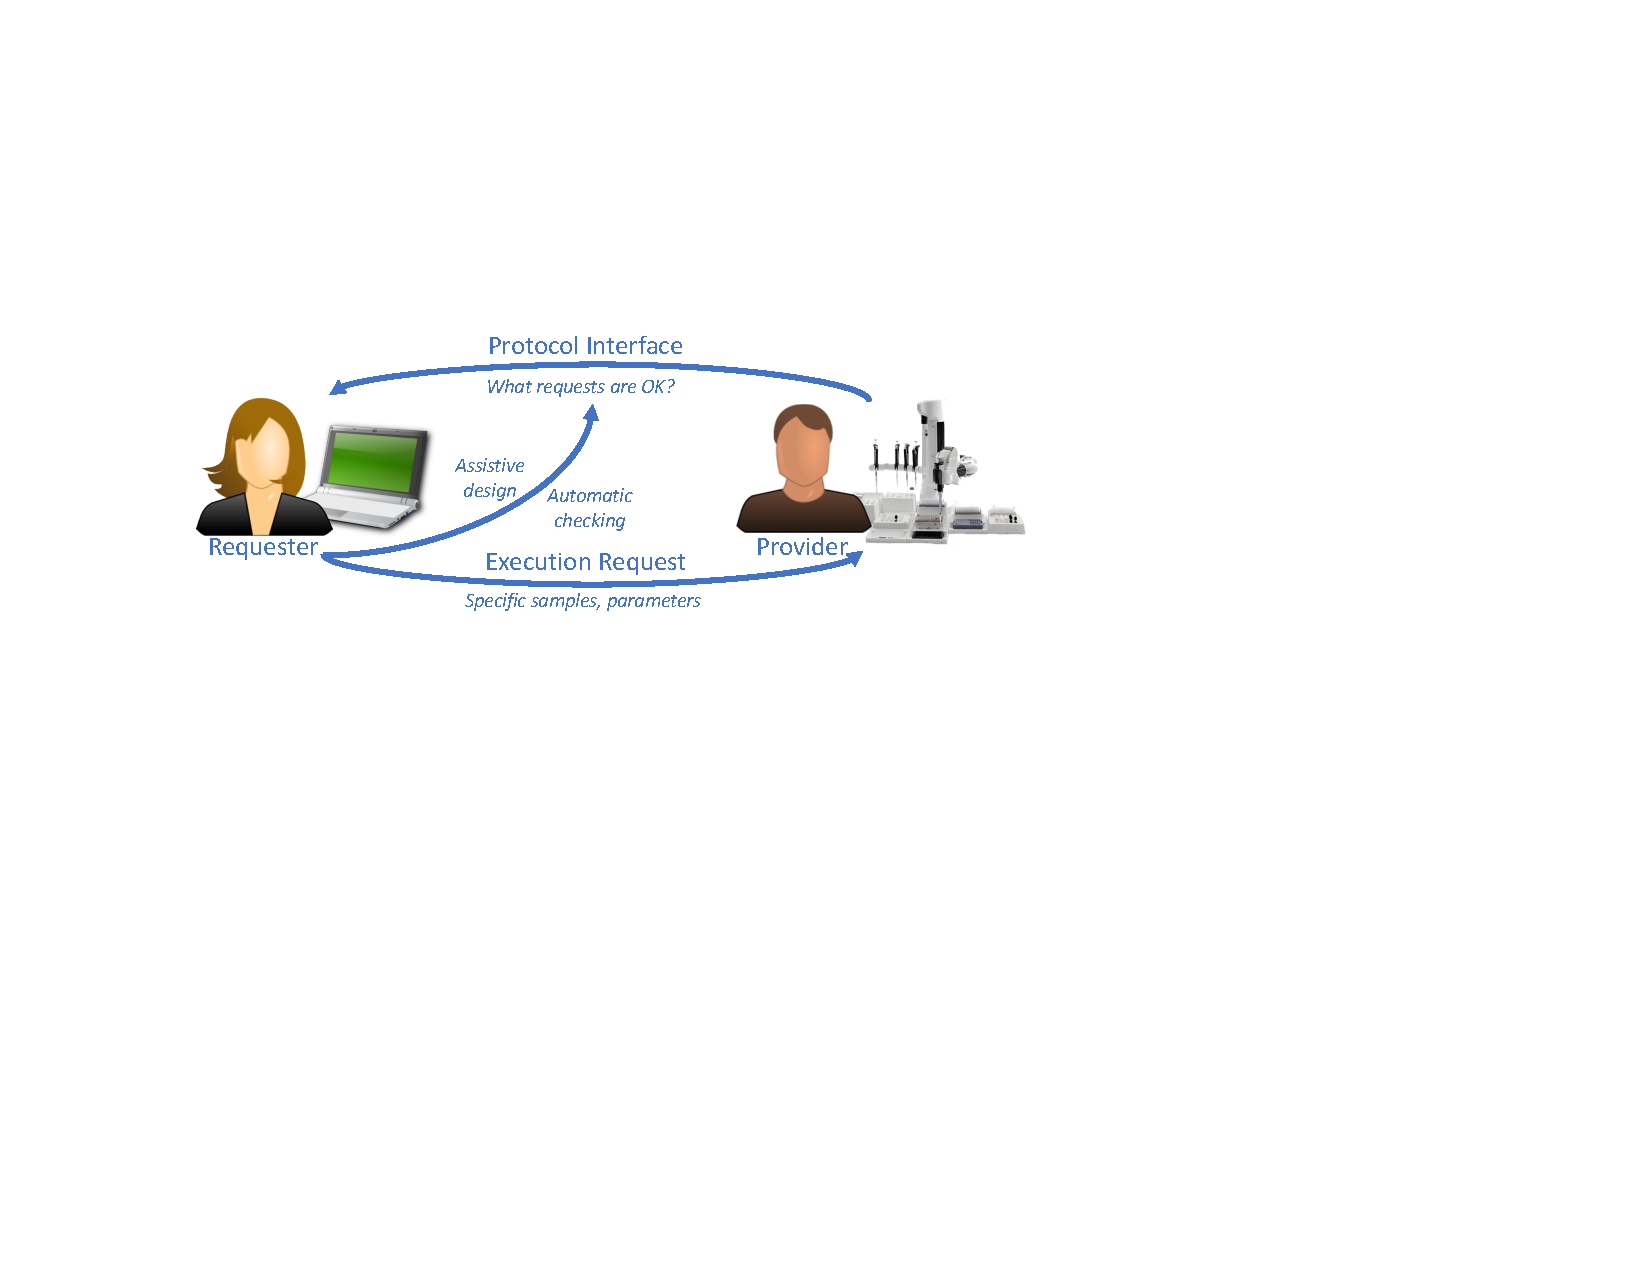
\includegraphics[width=0.8\textwidth]{figures/architecture.pdf}
\caption{OPIL connects experiment providers and requesters.}
\label{f:sequence}
\end{figure}

The Open Protocol Interface Language (OPIL) aims to address this problem by providing a data model to connect experiment providers and requesters.
Using OPIL, an experiment provider can provide a precise description of the protocols they offer, in terms of the options and constraints on the types of requests that can be made.
A requester can then use these interface descriptions to request the execution of a protocol on a specific set of samples with particular parameters.
OPIL can be applied both to automated protocols (e.g., via laboratory robotics or microfluidics) as well as to traditional human-executed ``paper'' protocols.

Where possible, OPIL builds on other existing standards.
In particular, OPIL uses the Synthetic Biology Open Language (SBOL) version 3~\citep{SBOL3} to describe biological samples in terms of combinations of strains, media, etc., and uses the Ontology of Units of Measure (OM) (\url{http://www.ontology-of-units-of-measure.org/resource/om-2}) to describe parameters with physical units.
Like these other standards, OPIL uses existing Semantic Web practices and resources, such as \emph{Uniform Resource Identifiers} (\opil{URI}s) and ontologies, to unambiguously identify and define biological system elements,
and to provide serialization formats for encoding this information in electronic data files.
This approach also allows OPIL to be extended with additional custom information for particular uses and deployments.

Note, however, that OPIL intentionally does not provide details about how the protocol works or guarantees about transfer or replicability of protocol executions. 
Likewise, OPIL is agnostic to any details of computer networking used to discover protocols or actually send requests.
OPIL focuses only on representing the minimal information for an unambiguous communication about requests to execute an offered protocol.



%% % -----------------------------------------------------------------------------
\section{Overview of OPIL}
% % -----------------------------------------------------------------------------

In OPIL, a protocol is an activity that is configured with certain parameters and applied to a set of biological samples in order to produce a set of measurements by particular instruments at particular times, as illustrated in \ref{f:overview}.
An \opil{ExperimentalRequest} specifies a particular set of \opil{ParameterValue}s, \opil{SampleSet}s, and \opil{Measurement}s to be carried out. 
A \opil{ProtocolInterface} specifies which \opil{ExperimentalRequest}s are allowed for a given protocol with a parallel construction of \opil{Parameter}s, \opil{SampleSet}s, and \opil{MeasurementType}s

\begin{figure}[ht]
\begin{center}
  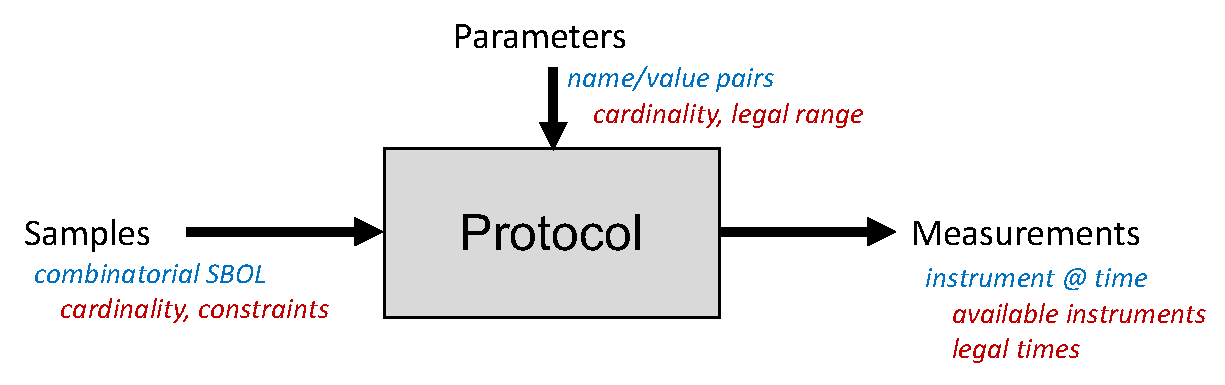
\includegraphics[scale=0.75]{figures/overview.pdf}
\caption{OPIL describes a request (blue) to execute a protocol in terms of samples, parameters, and measurements. 
A protocol interface (red) specifies what sorts of execution requests are allowed for that protocol.}
\label{f:overview}
\end{center}
\end{figure}

For example, consider a lab that is offering a multi-day bacterial protocol that might be described in prose as follows:
\begin{quote}
``Run either B. subtilis or E. coli samples in any media with up to 2 inducers for 1 to 4 days, sampling with a flow cytometer no more than once every 12 hours, and have the option of taking one RNAseq measurement. Culturing temperature is normally 37 C but can be set anywhere between 20 and 40 C.''
\end{quote}
These constraints could be encoded into a \opil{ProtocolInterface} by dividing them up as follows:
\begin{itemize}
\item Using \opil{SampleSet} objects: any {\it B. subtilis} or {\it E. coli} strain in any media, with up to 2 inducers.
\item Using \opil{Parameter} objects: run for 1-4 days, culture between 20-40 C with a default of 37 C.
\item Using \opil{MeasurementType} objects: any number of flow cytometer samples at least 12 hours apart, zero or one RNAseq measurement at any time.
\end{itemize}

An experimentalist who wishes to use this protocol might want to make a request such as the following:
\begin{quote}
``Please run all combinations of strains X and Y in media A, B, and C with 0, 0.1, 0.2, 0.5, and 1.0 uM arabinose. Run for 3 days with flow cytometry at hours 12, 30, 48, and 70. Culture at 27 C.''
\end{quote}
These specifies could be encoded into an \opil{ExperimentalRequest} by dividing them up as follows:
\begin{itemize}
\item Using \opil{SampleSet} objects: all combinations of strains X and Y in media A, B, and C with 0, 0.1, 0.2, 0.5, and 1.0 uM arabinose.
\item Using \opil{ParameterValue} objects: run for 3 days, culture at 27 C.
\item Using \opil{Measurement} objects: flow cytometry at hours 12, 30, 48, and 70.
\end{itemize}

The next sections provide complete definitions and details for all of these classes, along with more examples of their use.


%% -----------------------------------------------------------------------------
\section{Conventions}
% -----------------------------------------------------------------------------

This section provides some preliminary information to aid in the understanding of the specification.
The SBOL data model is specified using Unified Modeling Language (UML) 2.0 diagrams \href{http://www.omg.org/spec/UML/2.0/}{(OMG 2005)}. This section reviews terminology conventions, the basics of UML diagrams, and our naming conventions.

\subsection{Terminology Conventions}

This document indicates requirement levels using the controlled vocabulary specified in \href{https://tools.ietf.org/html/rfc2119}{IETF RFC 2119}.
In particular, the key words ``MUST'', ``MUST NOT'', ``REQUIRED'', ``SHALL'', ``SHALL NOT'', ``SHOULD'', ``SHOULD NOT'', ``RECOMMENDED'', ``MAY'', and ``OPTIONAL'' in this document are to be interpreted as described in RFC 2119.

\begin{itemize}
\item The words ``MUST'', ``REQUIRED'', or ``SHALL'' mean that the item is an absolute requirement.
\item The phrases ``MUST NOT'' or ``SHALL NOT'' mean that the item is an absolute prohibition.
\item The word ``SHOULD'' or the adjective ``RECOMMENDED'' mean that there might exist valid reasons in particular circumstances to ignore a particular item, but the full implications need to be understood and carefully weighed before choosing a different course.
\item The phrases ``SHOULD NOT'' or ``NOT RECOMMENDED'' mean that there might exist valid reasons in particular circumstances when the particular behavior is acceptable or even useful, but the full implications needs to be understood and the case carefully weighed before implementing any behavior described with this label.
\item The word ``MAY'' or the adjective ``OPTIONAL'' mean that an item is truly optional.
\end{itemize}

\subsection{UML Diagram Conventions}
\label{sec:umldiagrams}

The types of data modeled by OPIL are commonly referred to as {\em classes}, especially when discussing the details of software implementation. Each OPIL class can be instantiated by many OPIL objects. These objects MAY contain data that differ in content, but they MUST agree on the type and form of their data as dictated by their common class. Classes are represented in UML diagrams as rectangles labeled at the top with class names (see \ref{fig:uml_sampler} for examples).

\begin{figure}[ht]
\begin{center}
  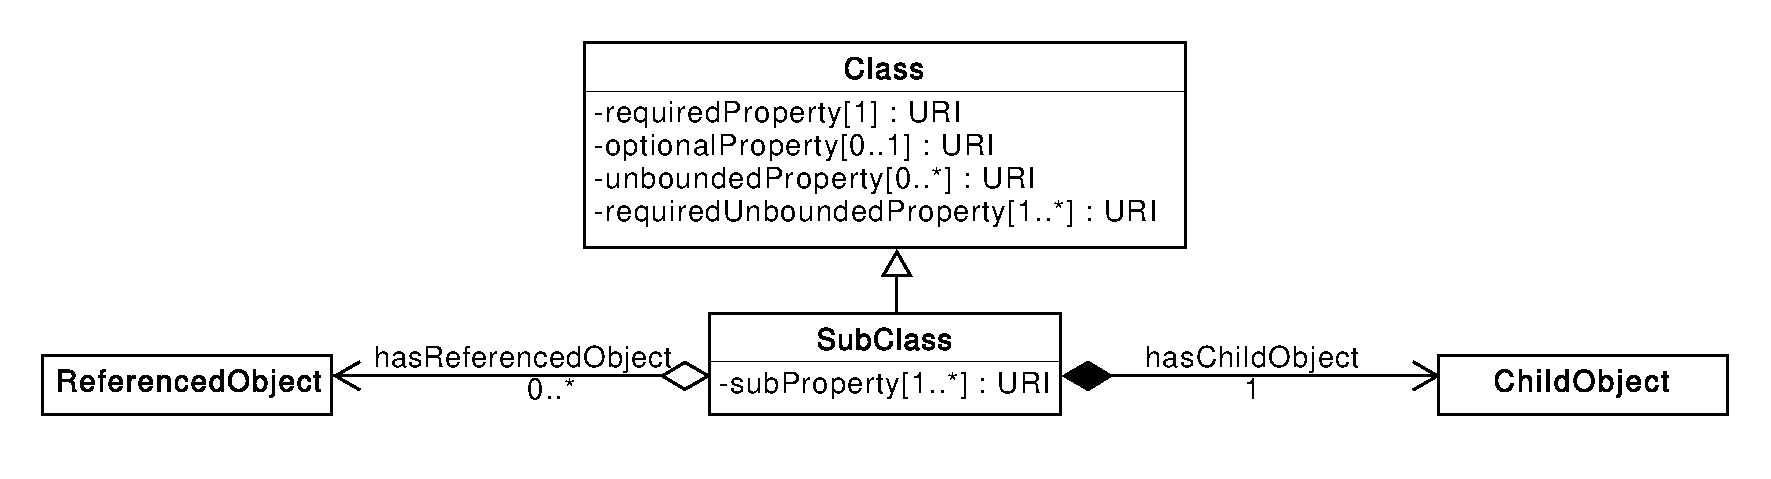
\includegraphics[width=\textwidth]{figures/uml_sampler.pdf}
\caption{Examples of UML diagram conventions used in this document}
\label{fig:uml_sampler}
\end{center}
\end{figure}

Classes can be connected to other classes by association properties, which are represented in UML diagrams as arrows. These arrows are labeled with data cardinalities in order to indicate how many values a given association property can possess (see below). The remaining (non-association) properties of a class are listed below its name. Each of the latter properties is labeled with its data type and cardinality.

In the case of an association property, the class from which the arrow originates is the owner of the association property. A diamond at the origin of the arrow indicates the type of association.
Open-faced diamonds indicate shared aggregation, also known as a reference, in which the owner of the association property exists independently of its value.

By contrast, filled diamonds indicate composite aggregation, also known as a part-whole relationship, in which the value of the association property MUST NOT exist independently of its owner.
In addition, in the OPIL data model, it is REQUIRED that the value of each composite aggregation property is a unique OPIL object (that is, not the value for more than one such property).
Note that in all cases, composite aggregation is used in such a way that there SHOULD NOT be duplication of such objects.
Such objects are also commonly referred to as ``child'' objects, and their owning objects as ``parent'' objects.

All OPIL properties are labeled with one of several restrictions on data cardinality. These are:

\begin{itemize}

\item $1$ - REQUIRED: there MUST be exactly one value for this property.

\item $0 \ldots 1$ - OPTIONAL: there MAY be a single value for this property, or it MAY be absent.

\item $0 \ldots *$ - zero or more: there MAY be any number of values for this property, including none.

\item $1 \ldots *$ - REQUIRED, one or more: there MAY be any number of values for this property, as long as there is at least one.

\item $n \ldots *$ - at least: there MUST be at least $n$ values for this property.

\end{itemize}

Finally, classes can inherit the properties of other classes. Inheritance relationships are represented in UML diagrams as open-faced, triangular arrows that point from the inheriting class to the inherited class. Some classes in the OPIL data model cannot be instantiated as objects and exist only to group common properties for inheritance. These classes have italicized names and are known as abstract classes.

\subsection{Naming and Typographic Conventions}
\label{sec:nameconventions}

OPIL classes are named using upper ``camel case,'' meaning that each word is capitalized and all words are run together without spaces, e.g., \opil{ProtocolInterface}.
Properties, on the other hand, are named using lower camel case, meaning that they begin lowercase but if they consist of multiple words, all words after the first begin with an uppercase letter (e.g., \opil{hasParameter}).

OPIL properties are always given singular names irrespective of their cardinality, e.g., \opil{hasParameter} is used rather than \opil{hasParameters} even though a \opil{ProtocolInterface} can have multiple parameters.
This is because each relation can potentially stand on its own, irrespective of the existence of others in the set.

Two conventions are used for property names, {\tt name} and {\tt hasName}.  
When a property is pointing to a class using the same name, it uses the {\tt hasName} convention (e.g., the \opil{ProtocolInterface} class uses \opil{hasParameter} to point to a \opil{Parameter} object).
When the property uses a different name than the class of the object it points to, it uses the {\tt name} convention instead (e.g., the \opil{MeasurementType} class uses \opil{minInterval} to point to a \opil{Measure} object).





%
\section{OPIL Data Model}\label{sec:model}

The section describes the OPIL data model in detail.  
OPIL classes are in general organized in pairs, one for specifying the interface to a protocol, the other for making requests to execute protocol via that interface.
As such, this section is also organized in pairs, first each interface class, then the complementary request class.

\todo[inline]{Change PI SampleSet to a new FactorSpace class?}

\subsection{ProtocolInterface}
\label{sec:ProtocolInterface}

The \opil{ProtocolInterface} class represents a protocol that is make available for use in requests for experiments.

\begin{figure}[ht]
\begin{center}
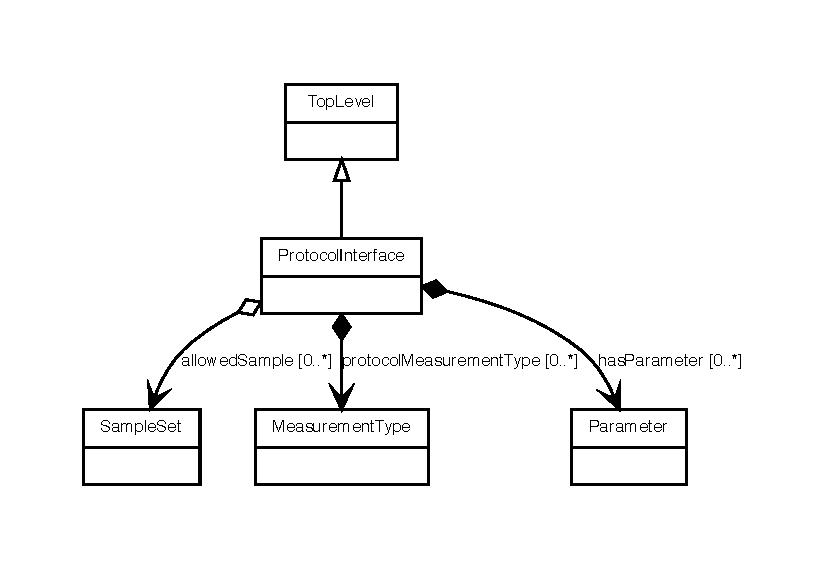
\includegraphics[scale=0.8]{figures/ProtocolInterface}
\caption[]{Diagram of the \opil{ProtocolInterface} class and its associated properties}
\label{uml:ProtocolInterface}
\end{center}
\end{figure}

\begin{itemize}
\item \label{sec:hasSampleSet}
The \opil{hasSampleSet} property MAY contain any number of \opil{URI}s, each of which refers to a \opil{SampleSet} object that describes a range of sample designs allowed for this protocol.
Any sample design whose properties fall into the range defined for any such \opil{SampleSet} SHOULD be accepted for execution of the protocol.
For example, a sample set might indicate that a protocol is intended for use with any strain of {\it E. coli} in any growth media with a concentration of one small-molecule inducer at a concentration between 0 and 1 $\mu$M.

\item \label{sec:hasParameter}
The \opil{hasParameter} property MAY contain any number of \opil{URI}s, each of which refers to a \opil{Parameter} object that describes one of the global parameters used to control the behavior of the protocol. 
For example, a \opil{Parameter} might be used for indicating the range of temperatures that can be requested for a culturing stage or the range of speeds for centrifuging.

\item \label{sec:hasMeasurementType}
The \opil{hasMeasurementType} property MAY contain any number of \opil{URI}s, each of which refers to a \opil{MeasurementType} object that describes a type of instrument that can be used to produce data from this protocol.
For example, a \opil{MeasurementType} might indicate that the protocol can read absorbance from a plate reader up to once every 10 minutes.
\end{itemize}

\subsection{ExperimentalRequest}
\label{sec:ExperimentalRequest}

The \opil{ExperimentalRequest} class is used to describe requests to actually run a particular protocol.

\begin{figure}[ht]
\begin{center}
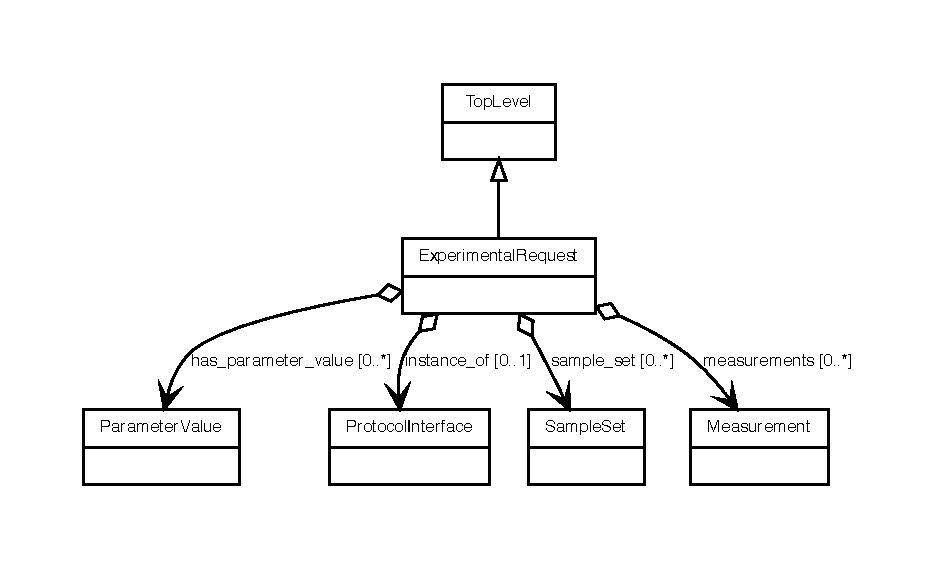
\includegraphics[scale=0.8]{figures/ExperimentalRequest}
\caption[]{Diagram of the \opil{ExperimentalRequest} class and its associated properties}
\label{uml:ExperimentRequest}
\end{center}
\end{figure}

\begin{itemize}
\item \label{sec:ER:instanceOf}
The \opilmult{ER:instanceOf}{instanceOf} property is REQUIRED and MUST contain a single \opil{URI} that refers to the \opil{ProtocolInterface} describing the protocol to be run.

\item \label{sec:hasSampleSet}
The \opil{hasSampleSet} property MAY contain any number of \opil{URI}s, each of which refers to a \opil{SampleSet} object that describes a collection of samples to be run through the experiment.
The total collection of samples requested is the union of all referred \opil{SampleSet} objects.

For example, a sample set might indicate that a protocol is intended for run in triplicate for a positive control strain, negative control strain, and four experimental strains, each at five different levels of inducer and in three different types of media (270 samples), and a second separate sample set might be used to request two replicates each of media-only control for each of the three media (6 samples), for a total of 276 samples.

\item \label{sec:hasMeasurement}
The \opil{hasMeasurement} property MAY contain any number of \opil{URI}s, each of which refers to a \opil{Measurement} object that sets the measurements to be collected during the execution of the protocol.
The total collection of measurements requested is the union of all referred \opil{SampleSet} objects.

For example, a \opil{Measurement} might be used to request plate reader absorbance data be collected at hours 0, 6, and 12, and a second \opil{Measurement} might be used to request that flow cytometry data be collected at hour 12.

\item \label{sec:hasParameterValue}
The \opil{hasParameterValue} property MAY contain any number of \opil{URI}s, each of which refers to a \opil{ParameterValue} object that sets one of the global parameters used to control the behavior of the protocol. 
To prevent conflicts between values, any two \opil{ParameterValue} object thus referred to MUST NOT be a \opil{valueOf} same \opil{Parameter} (e.g., culturing temperature cannot simultaneously be both 30 and  37 degrees Celsius).

For example, a \opil{ParameterValue} might be used to request that culturing temperature be set to 37 degrees Celsius and another used to set centrifuging to 5000 rpm.

\end{itemize}



\subsection{SampleSet}
\label{sec:SampleSet}

The \opil{SampleSet} class is an extension of \sbol{CombinatorialDerivation}, which adds the information of how many replicates should be executed for each specified sample in the combinatorial collection.

\begin{figure}[ht]
\begin{center}
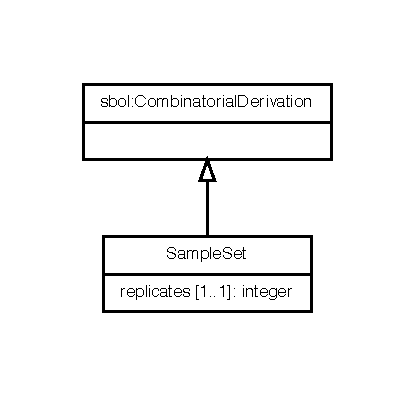
\includegraphics[scale=0.8]{figures/SampleSet}
\caption[]{Diagram of the \opil{SampleSet} class and its associated properties}
\label{uml:SampleSet}
\end{center}
\end{figure}

\begin{itemize}
\item \label{sec:replicates}
The \opil{replicates} property is REQUIRED and MUST contain a single positive \opil{integer} that indicates the number of replicates of each sample that should be run.
\end{itemize}


\subsection{MeasurementType}
\label{sec:MeasurementType}

The \opil{MeasurementType} class is used to indicate when and how often a particular modality of measurement is allowed to be used.
For example, it might be used to say that plate reader data is required to be taken, and that it can be taken up to three times in the range of 12 to 24 hours, no more frequently than once per hour.

\begin{figure}[ht]
\begin{center}
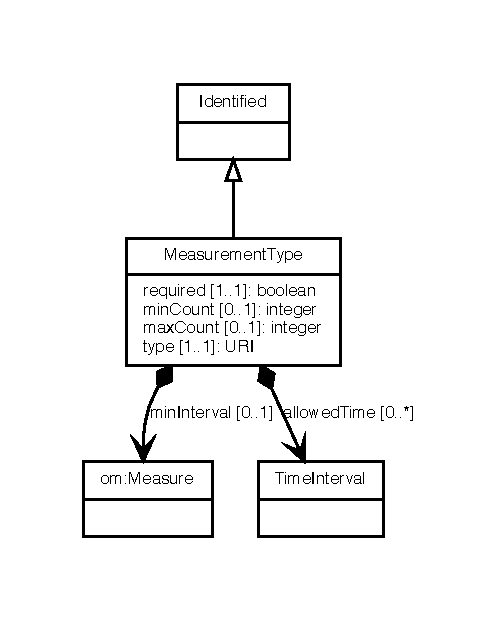
\includegraphics[scale=0.8]{figures/MeasurementType}
\caption[]{Diagram of the \opil{MeasurementType} class and its associated properties}
\label{uml:MeasurementType}
\end{center}
\end{figure}

\todo[inline]{Should we delete the required field, as redundant with minCount?}

\begin{itemize}
\item \label{sec:type}
The \opil{type} property is REQUIRED and MUST contain a \opil{URI} indicating the nature of the measurement being indicated.
When possible, this value SHOULD be drawn from the NCIT ontology's Instrumentation (\url{https://identifiers.org/NCIT:C16742}) or Laboratory Procedure (\url{https://identifiers.org/C25294}) branch.
A list of RECOMMENDED terms for common assays is provided in \ref{tbl:measurement_types}.

\item \label{sec:required}
The \opil{required} property is REQUIRED and MUST contain a \opil{boolean} indicating whether this type of measurement must be used during the execution of the protocol. 
For example, a protocol might always produce plate reader measurements (\opil{required} is true), but have proteomics optional (\opil{required} is false).

\item \label{sec:minCount}
The \opil{minCount} property is OPTIONAL and MAY contain a non-negative \opil{integer} indicating that this \\\opil{MeasurementType} MUST be requested at least the indicated number of times.
If \opil{minCount} is not set, it is treated as zero (or one if \opil{required} is true).
\opil{minCount} must be less than or equal to \opil{maxCount}.

\item \label{sec:maxCount}
The \opil{maxCount} property is OPTIONAL and MAY contain a non-negative \opil{integer} indicating that this \\\opil{MeasurementType} MUST NOT be requested more than the indicated number of times.
If \opil{maxCount} is not set, it is treated as infinity.
\opil{maxCount} must be greater than or equal to \opil{minCount}.


\item \label{sec:minInterval}
The \opil{minInterval} property is OPTIONAL and MAY contain a \opil{URI} referring to a \om{Measure} with a time duration unit indicating the minimum time between two subsequent measurements taken with this modality.
For example, setting \opil{minInterval} to a \om{Measure} specifying one hour would indicate that no two times when this \opil{MeasurementType} is requested may be less than one hour apart.
If \opil{minInterval} is not set, it is treated as zero.

\item \label{sec:allowedTime}
The \opil{allowedTime} property MAY contain any number of \opil{URI}s, each referring to a \opil{TimeInterval} that specifies a range of valid times.
The total set of valid times is the union of all such \opil{TimeInterval}s.
For example, one \opil{TimeInterval} could be used to indicate that the plate reader can be used right at the beginning of the protocol (time 0 hours), then again during the interval of 12 to 24 hours after it began.
If \opil{allowedTime} is not set, then all times are allowed.
\end{itemize}

\begin{table}[ht]
  \begin{edtable}{tabular}{ll}
    \toprule
    \textbf{Measurement Type} & \textbf{URI for NCIT Term} \\
    \midrule
    Flow cytometer & \url{https://identifiers.org/NCIT:C78806}\\
    Microplate reader & \url{https://identifiers.org/NCIT:C70661}\\
    RNAseq & \url{https://identifiers.org/NCIT:C124261}\\
    Fluorescence Microscopy & \url{https://identifiers.org/NCIT:C16856}\\
    \bottomrule
  \end{edtable}
  \caption{Partial list of NCIT terms to specify common assays using the \opil{type} property of a \opil{MeasurementType}}.
 \label{tbl:measurement_types}
\end{table}


\subsubsection{TimeInterval}
\label{sec:TimeInterval}

\todo[inline]{Fold in with factor space, if we do that?}

\opil{TimeInterval} is used for specifying valid ranges of time in which a measurement is allowed to be taken.
For example, it might be used to say that a measurement can be taken anywhere in the range of 12 to 24 hours, or might be used to say that measurements cannot be taken before hour 3.

\begin{figure}[ht]
\begin{center}
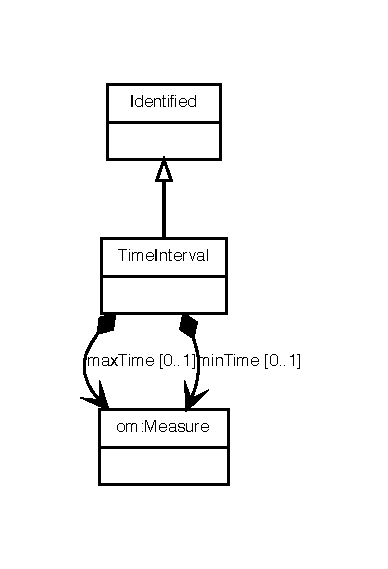
\includegraphics[scale=0.8]{figures/TimeInterval}
\caption[]{Diagram of the \opil{TimeInterval} class and its associated properties}
\label{uml:TimeInterval}
\end{center}
\end{figure}

\begin{itemize}
\item \label{sec:minTime}
The \opil{minTime} property is OPTIONAL and MAY contain a \opil{URI} referring to a \om{Measure} with a time duration unit.
If \opil{minTime} is not set, it is treated as zero.
\opil{minTime} must be less than or equal to \opil{maxTime}.

\item \label{sec:maxTime}
The \opil{maxTime} property is OPTIONAL and MAY contain a \opil{URI} referring to a \om{Measure} with a time duration unit.
If \opil{maxTime} is not set, it is treated as infinity.
\opil{maxTime} must be greater than or equal to \opil{minTime}.
\end{itemize}


\subsection{Measurement}
\label{sec:Measurement}

The \opil{Measurement} class is used to request that a particular measurement be performed at certain times.
For example, it might be used to request that a plate reader be used at hours 0, 6, and 12.

\begin{figure}[ht]
\begin{center}
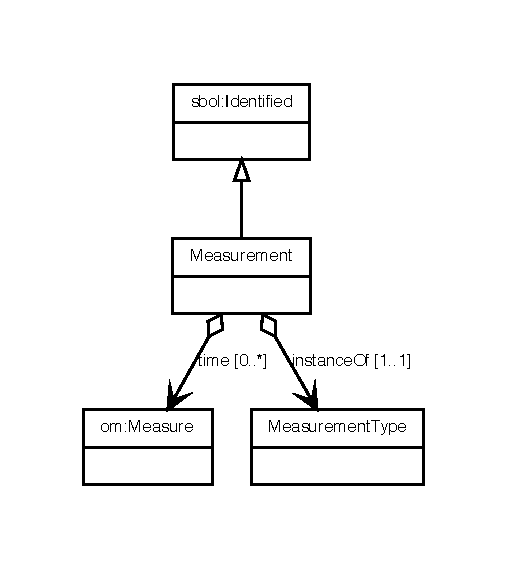
\includegraphics[scale=0.8]{figures/Measurement}
\caption[]{Diagram of the \opil{Measurement} abstract class and its associated properties}
\label{uml:Measurement}
\end{center}
\end{figure}

\begin{itemize}
\item \label{sec:M:instanceOf}
The \opilmult{M:instanceOf}{instanceOf} property is REQUIRED and MUST contain a single \opil{URI} that refers to the \opil{MeasurementType} describing the measurement to be taken.

\item \label{sec:time}
The \opil{time} property MAY contain any number of \opil{URI}s, each referring to a \om{Measure} with a time unit.
\end{itemize}





\subsection{Parameter}
\label{sec:Parameter}

\todo[inline]{Should type be transformed from class type to a field on Parameter, except for the ones that actually have additional fields? This would simplify type-matching validation rules, but add complexity to knowing when an extension is necessary. The EnumeratedParameter allowedValue field could certainly generalize to any. Likewise, the min and max could be generalized for any orderable type (and maybe folded in with factor spaces, if we do that).}
\todo[inline]{I think we need an additional field here to indicate whether a parameter is required or not}

\opil{Parameter} is an abstract class that represents any sort of global setting that may be provided to configure the execution of a protocol.
The subclasses of \opil{Parameter} are used to indicate different types of value to be set, such as Booleans, integers, and measures (i.e., floating point values with units).

This is a catch-all class intended for capturing any information that cannot be systematized in terms of \opil{SampleSet} and \opil{Measurement} information, and thus SHOULD NOT be used to represent anything that can be well-represented using those classes.

For example, a \opil{Parameter} can be used to determine whether an optional post-culturing dilution step should be executed.
A \opil{Parameter} SHOULD NOT be used to determine which culture media should be used in a sample (since that can be represented well via \opil{SampleSet}) or to indicate whether samples should be evaluated with an optional proteomics step (since that can be represented well via \opil{Measurement}).



\begin{figure}[ht]
\begin{center}
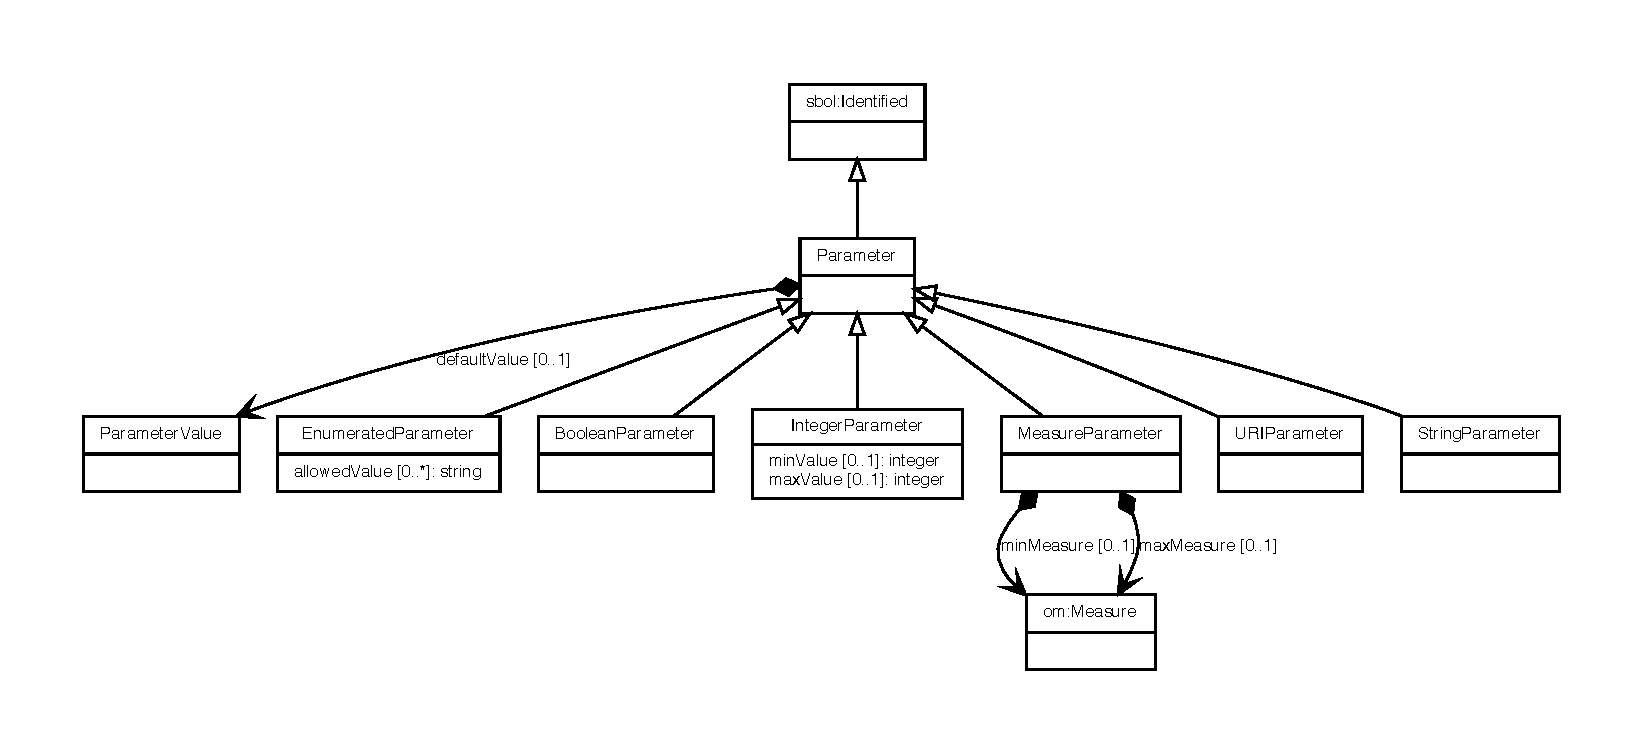
\includegraphics[scale=0.6]{figures/Parameter_definition_and_abstraction}
\caption[]{Diagram of the \opil{Parameter} abstract class and its associated properties and subclasses}
\label{uml:Parameter}
\end{center}
\end{figure}

\begin{itemize}
\item \label{sec:defaultValue}
The \opil{defaultValue} property is OPTIONAL and MAY contain a single \opil{URI} that refers to a \opil{ParameterValue} that provides a default value for the parameter in the case that it is not set.
\end{itemize}


\subsubsection{BooleanParameter}
\label{sec:BooleanParameter}

{\em \opil{BooleanParameter} has no additional properties.}

\subsubsection{EnumeratedParameter}
\label{sec:EnumeratedParameter}

\begin{itemize}
\item \label{sec:allowedValue}
The \opil{allowedValue} property MAY contain any number of \opil{string} values, indicating the legal values for this \opil{EnumeratedParameter}. 
For example, 
\end{itemize}

\subsubsection{IntegerParameter}
\label{sec:IntegerParameter}

\begin{itemize}
\item \label{sec:minValue}
The \opil{minValue} property is OPTIONAL and MAY contain an \opil{integer}.
If \opil{minValue} is not set, it is treated as negative infinity.
\opil{minValue} must be less than or equal to \opil{maxValue}.

\item \label{sec:maxValue}
The \opil{maxValue} property is OPTIONAL and MAY contain an \opil{integer}.
If \opil{maxValue} is not set, it is treated as infinity.
\opil{maxValue} must be greater than or equal to \opil{minValue}.
\end{itemize}

\subsubsection{MeasureParameter}
\label{sec:MeasureParameter}

\begin{itemize}
\item \label{sec:minMeasure}
The \opil{minMeasure} property is OPTIONAL and MAY contain a \opil{URI} referring to a \om{Measure}.
If \opil{minMeasure} is not set, it is treated as negative infinity.
\opil{minMeasure} must be less than or equal to \opil{maxMeasure}.

\item \label{sec:maxMeasure}
The \opil{maxMeasure} property is OPTIONAL and MAY contain a \opil{URI} referring to a \om{Measure}.
If \opil{maxMeasure} is not set, it is treated as infinity.
\opil{maxMeasure} must be greater than or equal to \opil{minMeasure}.
\end{itemize}

\subsubsection{StringParameter}
\label{sec:StringParameter}

{\em \opil{BooleanParameter} has no additional properties.}

\subsubsection{URIParameter}
\label{sec:URIParameter}

{\em \opil{BooleanParameter} has no additional properties.}


\subsection{ParameterValue}
\label{sec:ParameterValue}

\opil{ParameterValue} is an abstract class is used to set a parameter for a protocol to a particular value. 
The subclasses of \opil{ParameterValue} are used for different types of value to be set, such as Booleans, integers, and measures (i.e., floating point values with units).
For example, a \opil{MeasureValue} might be used to request that a centrifuging step be run at 5000 rpm.

\begin{figure}[ht]
\begin{center}
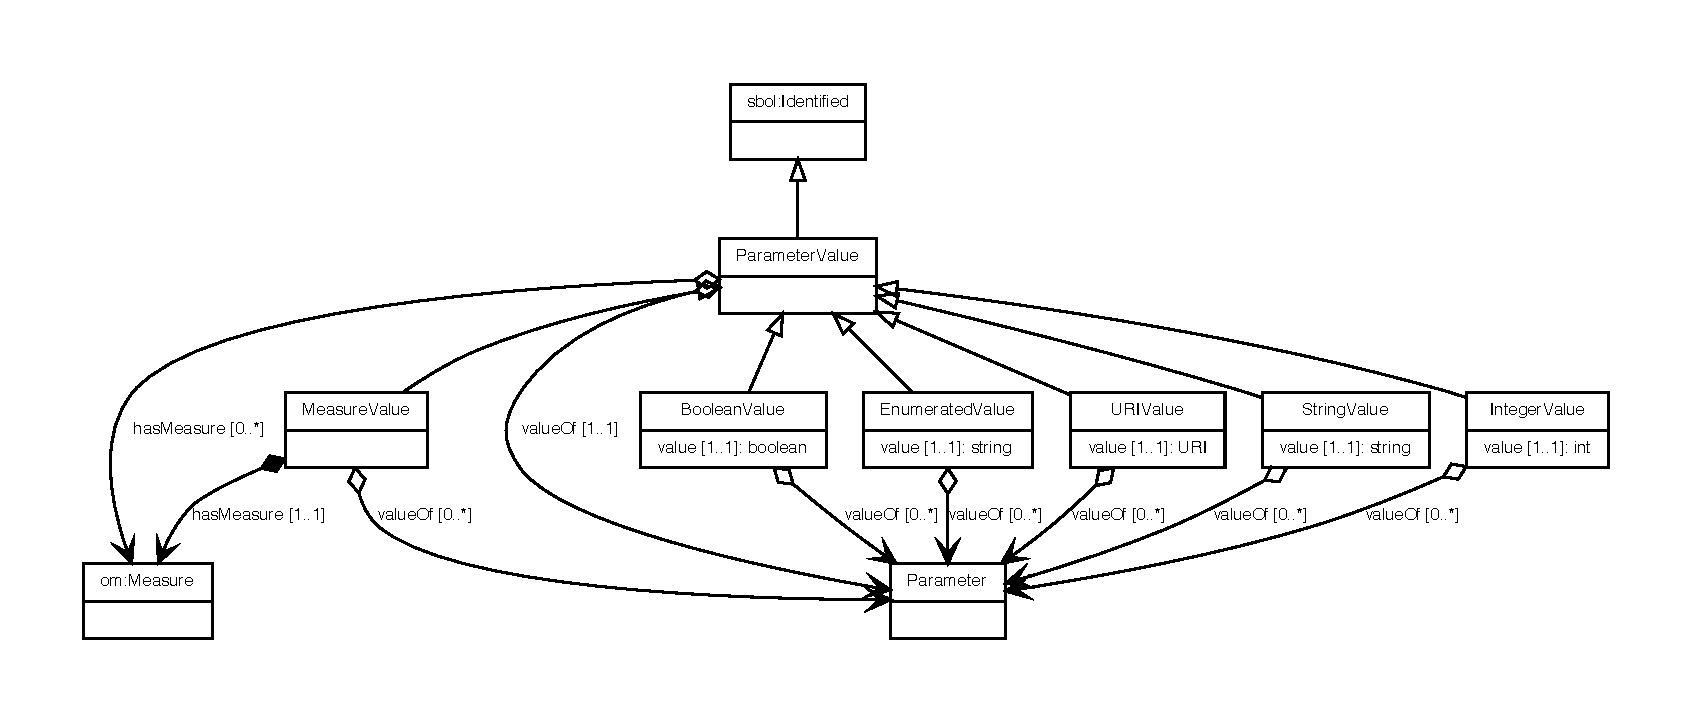
\includegraphics[scale=0.6]{figures/ParameterValue_definition_and_abstraction}
\caption[]{Diagram of the \opil{ParameterValue} abstract class and its associated properties and subclasses}
\label{uml:ParameterValue}
\end{center}
\end{figure}

\begin{itemize}
\item \label{sec:valueOf}
The \opil{valueOf} property is REQUIRED and MUST contain a single \opil{URI} that refers to the \opil{Parameter} describing the parameter being set.
The \opil{Parameter} MUST be of a corresponding class, e.g., a \opil{BooleanValue} must match a \opil{BooleanParameter}.
\end{itemize}


\subsubsection{BooleanValue}
\label{sec:BooleanValue}

\begin{itemize}
\item \label{sec:BP:value}
The \opilmult{BP:value}{value} property is REQUIRED and MUST contain a single \opil{boolean}.
\end{itemize}

\subsubsection{EnumeratedValue}
\label{sec:EnumeratedValue}

\begin{itemize}
\item \label{sec:EV:value}
The \opilmult{EV:value}{value} property is REQUIRED and MUST contain a single \opil{string} whose value is equal to one of the \opil{allowedValue} properties of the \opil{Parameter} referred to by the \opil{valueOf} property.
\end{itemize}


\subsubsection{IntegerValue}
\label{sec:IntegerValue}

\begin{itemize}
\item \label{sec:IV:value}
The \opilmult{IV:value}{value} property is REQUIRED and MUST contain a single \opil{integer}.
The value must be greater than or equal to that of the \opil{minValue} property (if set) of the \opil{Parameter} referred to by the \opil{valueOf} property, and less than or equal to the \opil{maxValue} property (if set).
\end{itemize}

\subsubsection{MeasureValue}
\label{sec:MeasureValue}

\begin{itemize}
\item \label{sec:hasValue}
The \opil{hasValue} property is REQUIRED and MUST contain a single \opil{URI} referring to a \om{Measure} object containing the value for the parameter.
The value of the linked \om{Measure} must be greater than or equal to that of the \opil{minMeasure} property (if set) of the \opil{Parameter} referred to by the \opil{valueOf} property, and less than or equal to the \opil{maxMeasure} property (if set).
\end{itemize}


\subsubsection{StringValue}
\label{sec:StringValue}

\begin{itemize}
\item \label{sec:SV:value}
The \opilmult{SV:value}{value} property is REQUIRED and MUST contain a single \opil{string}.
\end{itemize}


\subsubsection{URIValue}
\label{sec:URIValue}

\begin{itemize}
\item \label{sec:UV:value}
The \opilmult{UV:value}{value} property is REQUIRED and MUST contain a single \opil{URI}.
\end{itemize}












%\section{Serialization}
\label{sec:serialization}

In order for OPIL objects to be readily stored and exchanged, it is important that they are able to be {\em serialized}, i.e., converted to a sequence of bytes that can be stored in a file or exchanged over a network.  
%
To this end, OPIL builds upon the Resource Description Framework (RDF).  RDF is an abstract language for describing conceptual graph-oriented data models, and therefore does not mandate any specific serialization format.  Instead, a number of different serialization formats are provided as separate specifications, such as RDF/XML, N-Triples, JSON-LD, and Turtle.  These serialization formats are widely supported by RDF libraries such as rdflib for Python and Apache Jena for Java.

All OPIL libraries SHOULD support at least RDF/XML, N-Triples, JSON-LD, and Turtle.
Other OPIL tools SHOULD support at least one of these four formats.


\newpage
\bibliography{opil}

\appendix

%\input{examples}

\end{document}
